\section{Background and motivation for SSU-ALIGN}

\sft{ssu-align} is a freely available, open source software program
for creating large-scale alignments of small subunit ribosomal RNA
(SSU) using covariance models (CMs). The archaeal, bacterial,
and eukaryotic SSU CMs in \sft{ssu-align} are built from structural
seed alignments derived from Robin Gutell's Comparative RNA Website
(CRW) \cite{CannoneGutell02}. 

There are several outstanding software packages dedicated to SSU
alignment, including, but not limited to, \software{NAST} (used by the
\software{greengenes} database), \software{PyNast}, \software{SINA}
(used by the \software{silva} database), and \software{mothur}. 
\sft{ssu-align} has several features that distinguish it from these
programs: 

\begin{itemize}

\item \textbf{Structural alignments are calculated at roughly one
  second per sequence.}  

  CM alignment takes into account conserved sequence and well-nested
  structure. In the past, the slow speed of CM alignment (about 10
  minutes/sequence) has prevented their application to SSU alignment,
  but acceleration heuristics that take advantage of the high levels
  of sequence conservation in SSU \cite{Nawrocki09b} making
  large-scale SSU CM alignment more feasible. Other available methods
  do not explicitly take secondary structure into account during
  alignment.

\item \textbf{Masks for pruning ambiguously aligned columns are
  automatically generated.}
  
  CMs are probabilistic models that allow calculation of the posterior
  probability that each sequence nucleotide belongs in each column of the
  output alignment given the model. Regions of low posterior
  probabilities are indicative of high alignment ambiguity and
  should be pruned away (masked out) prior to phylogenetic
  inference. \sft{ssu-align} can automatically detect and remove
  these columns for any alignment it generates using the
  \prog{ssu-mask} program. The tutorial (section~\ref{sec:tutorial})
  contains an example. 

\item \textbf{Accurate alignments can be computed using seed
  alignments of less than one hundred sequences.}

  CMs built from small seed alignments of only dozens of sequences
  can achieve comparable accuracy to nearest-neighbor based alignment
  methods that use seed (reference) alignments of thousands or tens of
  thousands of sequences. This reduces the level of manual curation
  necessary for creating useful seeds, making it easy to extend
  \sft{ssu-align} by adding new seeds and corresponding CMs that cover
  specific phylogenetic ranges. For example, a
  \emph{Firmicute}-specific seed and model could be constructed to
  create large alignments for phylogenetic analysis of the \emph{Firmicute}
  bacterial phyla.

\end{itemize}

\subsection{Profile versus nearest neighbor alignment strategies}

Many existing methods for SSU alignment use a \emph{nearest-neighbor}
(NN) based alignment strategy: given a new target sequence to align,
each sequence in a reference alignment is evaluated to find one or
more nearest-neighbor template sequences that are most similar to the
target using a similarity metric such as sequence identity. An
alignment of the target sequence to its template(s) is then
computed, and this alignment is used to place the target within the
context of the full reference alignment (figure~\ref{fig:nnprof}.

In contrast \software{ssu-align} uses a profile-based alignment
strategy: each target sequence is aligned independently to a
statistical model called a profile
(figure~\ref{fig:nnprof}). \software{ssu-align} uses profiles called
covariance models (CMs) for alignment
%, which model both the conserved sequence and secondary structure of SSU
\footnote{\textsc{ssu-align} actually uses two types of profiles,
  CMs and profile HMMs, which model only conserved primary
  sequence. Profile HMMs are used to determine which domain each
  sequence belongs to, and then the corresponding domain-specific CM
  is used to align the sequence, as depicted in
  figure~\ref{fig:schematic}.}.
A comprehensive explanation of CMs is outside the scope of this
guide. Instead, a brief discussion of some of their relevant features
for using \textsc{SSU-ALIGN} and understanding its output is included
below. For more information on CMs see
\cite{Eddy94,Durbin98,Eddy02b,NawrockiEddy07,Nawrocki09,Nawrocki09b,KolbeEddy09}.

\begin{figure}
  \begin{center}
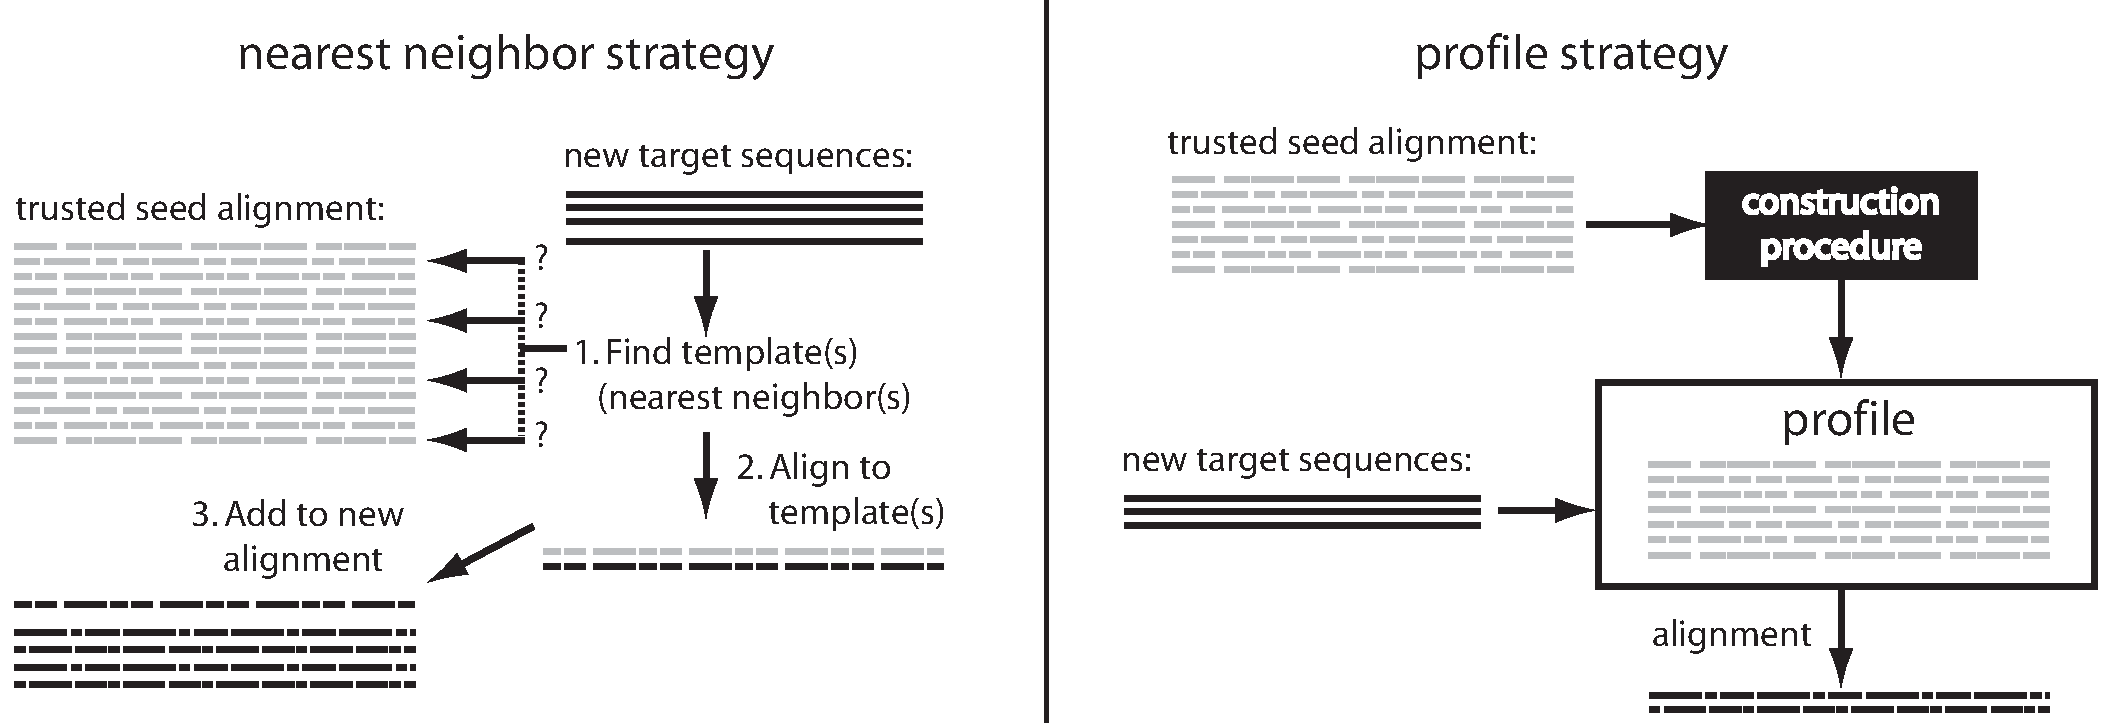
\includegraphics[width=6in]{Figures/nnprof}
  \end{center}
  \caption{Schematic of nearest-neighbor and
        profile based alignment strategies.}
  \label{fig:nnprof}
\end{figure}

A CM is a consensus model of the conserved sequence and secondary
structure of an RNA family that is built from a multiple sequence
alignment. This alignment is sometimes called the \emph{seed} or
\emph{training} alignment of the model. The seed alignment should
include a representative set of sequences from the family being
modeled and must include consensus structure annotation indicating
which positions in the alignment are basepaired to each other.  Given
a new target sequence, its best-scoring alignment to the CM can be
computed using a dynamic programming algorithm. Both primary
sequence conservation and secondary structure conservation between the target
and the model contribute to the alignment score.
%  that takes into account both the sequence and structure conservation in the

The default archaeal, bacterial, and eukaryotic CMs used by
\sft{ssu-align} have 1508, 1582, and 1881 consensus positions,
respectively. Any column for which fewer than 80\% of the sequences in
the seed alignment had gaps was defined as a consensus position when
the default models were constructed. The derivation of the three seed
alignments and the specific method used to build the models is
discussed in detail in section~\ref{sec:models} of this guide.

Profiles like CMs use position-specific scores learned from the seed
alignment for aligning each possible nucleotide in a target sequence
to each consensus position. Basepaired positions 
%For example, a consensus position that is
%100\% \prog{G} in the seed alignment will assign \prog{G} a high
%score and other nucleotides a low score, while a consensus position
%that is 25\% \prog{A}, \prog{C}, \prog{G} and \prog{U} will assign all
%four nucleotides marginal scores. 
A CM also contains position-specific scores for inserting nucleotides,
i.e. placing them in between two adjacent consensus positions, and deleting nucleotides,
i.e. aligning a consensus position to a gap in the sequence. 
%Whenever
%a sequence requires an insert after a consensus column, gaps must be
%added to accomodate that insert in the other sequences in the
%alignment.

\subsubsection{Profiles use position-specific scores}

The scores used when aligning sequences to a CM are position-specific
and are derived from the observed nucleotide distributions in the seed
alignment. As a simple example, consider the small structural RNA
family in figure~\ref{fig:seed-ex}. This RNA forms the simple stem-loop
structure shown on the right of the figure. The alignment is in
Stockholm format, which is explained more in the tutorial section. 
The \prog{\#=GC SS\_cons} line maps this structure onto the
alignment. Basepairs in this line are indicated by matching \prog{<}
with \prog{>}, just like matching parantheses in a mathematical
formula. When a CM is built from this seed alignment, each of the
columns that include fewer than 80\% gaps will become consensus
positions of the model. Basepaired positions will become consensus
basepairs, and other positions will be single-stranded consensus
positions. Each single-stranded consensus position of the model will
include scores for aligning to each of the four possible nucleotides:
\prog{A}, \prog{C}, \prog{G}, and \prog{U}, based on their frequency
in the corresponding position of the alignment. For example, column x,
which is 100\% \prog{G} in the seed alignment would assign high scores
to \prog{G} and low scores to all other nucleotides. In contrast,
column x, which includes two of each of the four nucleotides would
assign equal, marginal scores to all four nucleotides.
Importantly, basepaired positions will
assign scores to two nucleotides at once and so will include scores
for each of the 16 possible pairs of nucleotides. For example, the
-most pair is 100\% \prog{GC} in the seed alignment and so \prog{GC}
pairs in the target would receive high scores, while the other 15
possible pairs would receive low scores. In contrast, the -most
basepair includes two of each of the four possible Watson-Crick
basepairs: \prog{AU}, \prog{UA}, \prog{CG}, and \prog{GC}, and so
these four basepairs would receive high scores, while the other 12
possible pairs would receive lower scores. Additionally,
position-specific scores for inserting nucleotides are derived from
the alignment. Position x is the only one after which any insertions
occur in the alignment, and so its score for inserting residues would
be higher than the other positions. Similarly, the only deletions,
i.e. gaps in consensus positions occur in positions y and z, with one
occuring in y, and three in z. Consequently, the deletion score for
position z would be highest, with deletes in y receiving lower scores,
and all other positions receiving still lower scores
\footnote{This discussion
  purposefully omits precise mathematical formulas for brevity. For
  more detail on how the position-specific scores are calculated, see 
  \prog{Durbin98, Nawrocki09}.}. 

In contrast, nearest-neighbor based methods often do not use
position-specific scores. For example, if a single template sequence
is used there is no way for the method to distinguish the level of
conservation in different positions, and so the scores for aligning an
\prog{A}, \prog{C}, \prog{G}, and \prog{U} at each position is
identical.
%Notably, the nearest-neighbors-based \sft{sina} aligner
%used by the \sft{silva} database does not have this limitation as it
%uses up to 40 template sequences \cite{Pruesse07} to align each
%target. 
Pairwise alignment with position-independent scores is accurate when
the template is nearly identical to the target, but becomes more
difficult as that identity decreases. As a result, most
nearest-neighbor based methods use very large reference alignments
(thousands of sequences) to increase the probability that a nearly
identical template exists for any potential target. Curating and
ensuring the accuracy of such large reference alignments is a lot of
work. Seed alignments for profile-based methods on the other
traditionally include less than one hundred sequences \cite{Finn10,Gardner09}. 
%In fact, the
%\sft{pfam} and \sft{rfam} databases collectively include over 12,000
%separate seed alignments, the vast majority of which contain fewer
%than 100 sequences. 

\subsection{Two types of alignment columns: consensus and inserts}

Alignments created by \sft{ssu-align} will contain two types of
columns: consensus columns, that correspond to a consensus position of
the model, and insert columns, which include nucleotides
inserted between consensus positions of the model. These columns can
be distinguished based on the \prog{\#=GC RF} line in the alignment
files. Continuing with the small RNA example, figure~\ref{fig:toyex}
shows an alignment of 10 target sequences to the CM built from the
alignment in~\ref{fig:insert-ex}. Notice that the \prog{\#=GC RF} line
contains 12 nucleotides, one for each of the consensus columns in the model.
These are the highest scoring nucleotides at each position. Uppercase
letters in this line were highly conserved in the seed alignment,
lowercase letters were less well conserved.

Figure~\ref{fig:toyex} demonstrates two important caveats of
profile-based alignment by \sft{ssu-align}. 

\begin{enumerate}
\item 
Nucleotides in insert columns are simply inserted, not aligned.

You might have noticed that the nucleotides in the insert columns x
and x are obviously misaligned with respect to each other. This is
because \sft{ssu-align} does not align inserts. Instead, inserted
nucleotides are split in half, the left half is placed flush-left next
to nearest consensus column on the left (\prog{xx} in sequence x), and
the right half is placed flush-right next to the nearest consensus
column to the right (\prog{x} in sequence y). This is an important
limitation of profile-based alignment. A nearest-neighbor based
method might be able to correctly align nucleotides that would be
inserts for a profile. However, inserted positions
should be rare. Remember that consensus positions were defined as any
position that had a nucleotide in at least 20\% of the seed
sequences, so if the seed was representative the most common inserts
should only appear in about 20\% of sequences. And if the alignment will
eventually be used for phylogenetic inference, inserted columns should
be removed first anyway, and so are unimportant. This is discussed
further below in the section on masking alignments.

\item 
Deeper alignments tend to have more insert columns. 

Because the likelihood of a large insertion in at least one sequence
increases as more sequences are added, alignments of large numbers of
sequences (deep alignments) tend to have a lot of insert columns. In
fact, the number of insert columns can routinely be greater than the
number of consensus columns. This contrasts markedly with the popular
nearest-neighbor based aligners \sft{nast} and \sft{sina}, which
generate alignments of a fixed with (7,682 columns for \sft{nast} and
50,000 for \sft{sina}). However to guarantee a fixed width, \sft{nast}
must deliberately introduce errors in the alignment in some cases
\cite{DeSantis06}. 

\end{enumerate}

\begin{figure}
\begin{center}
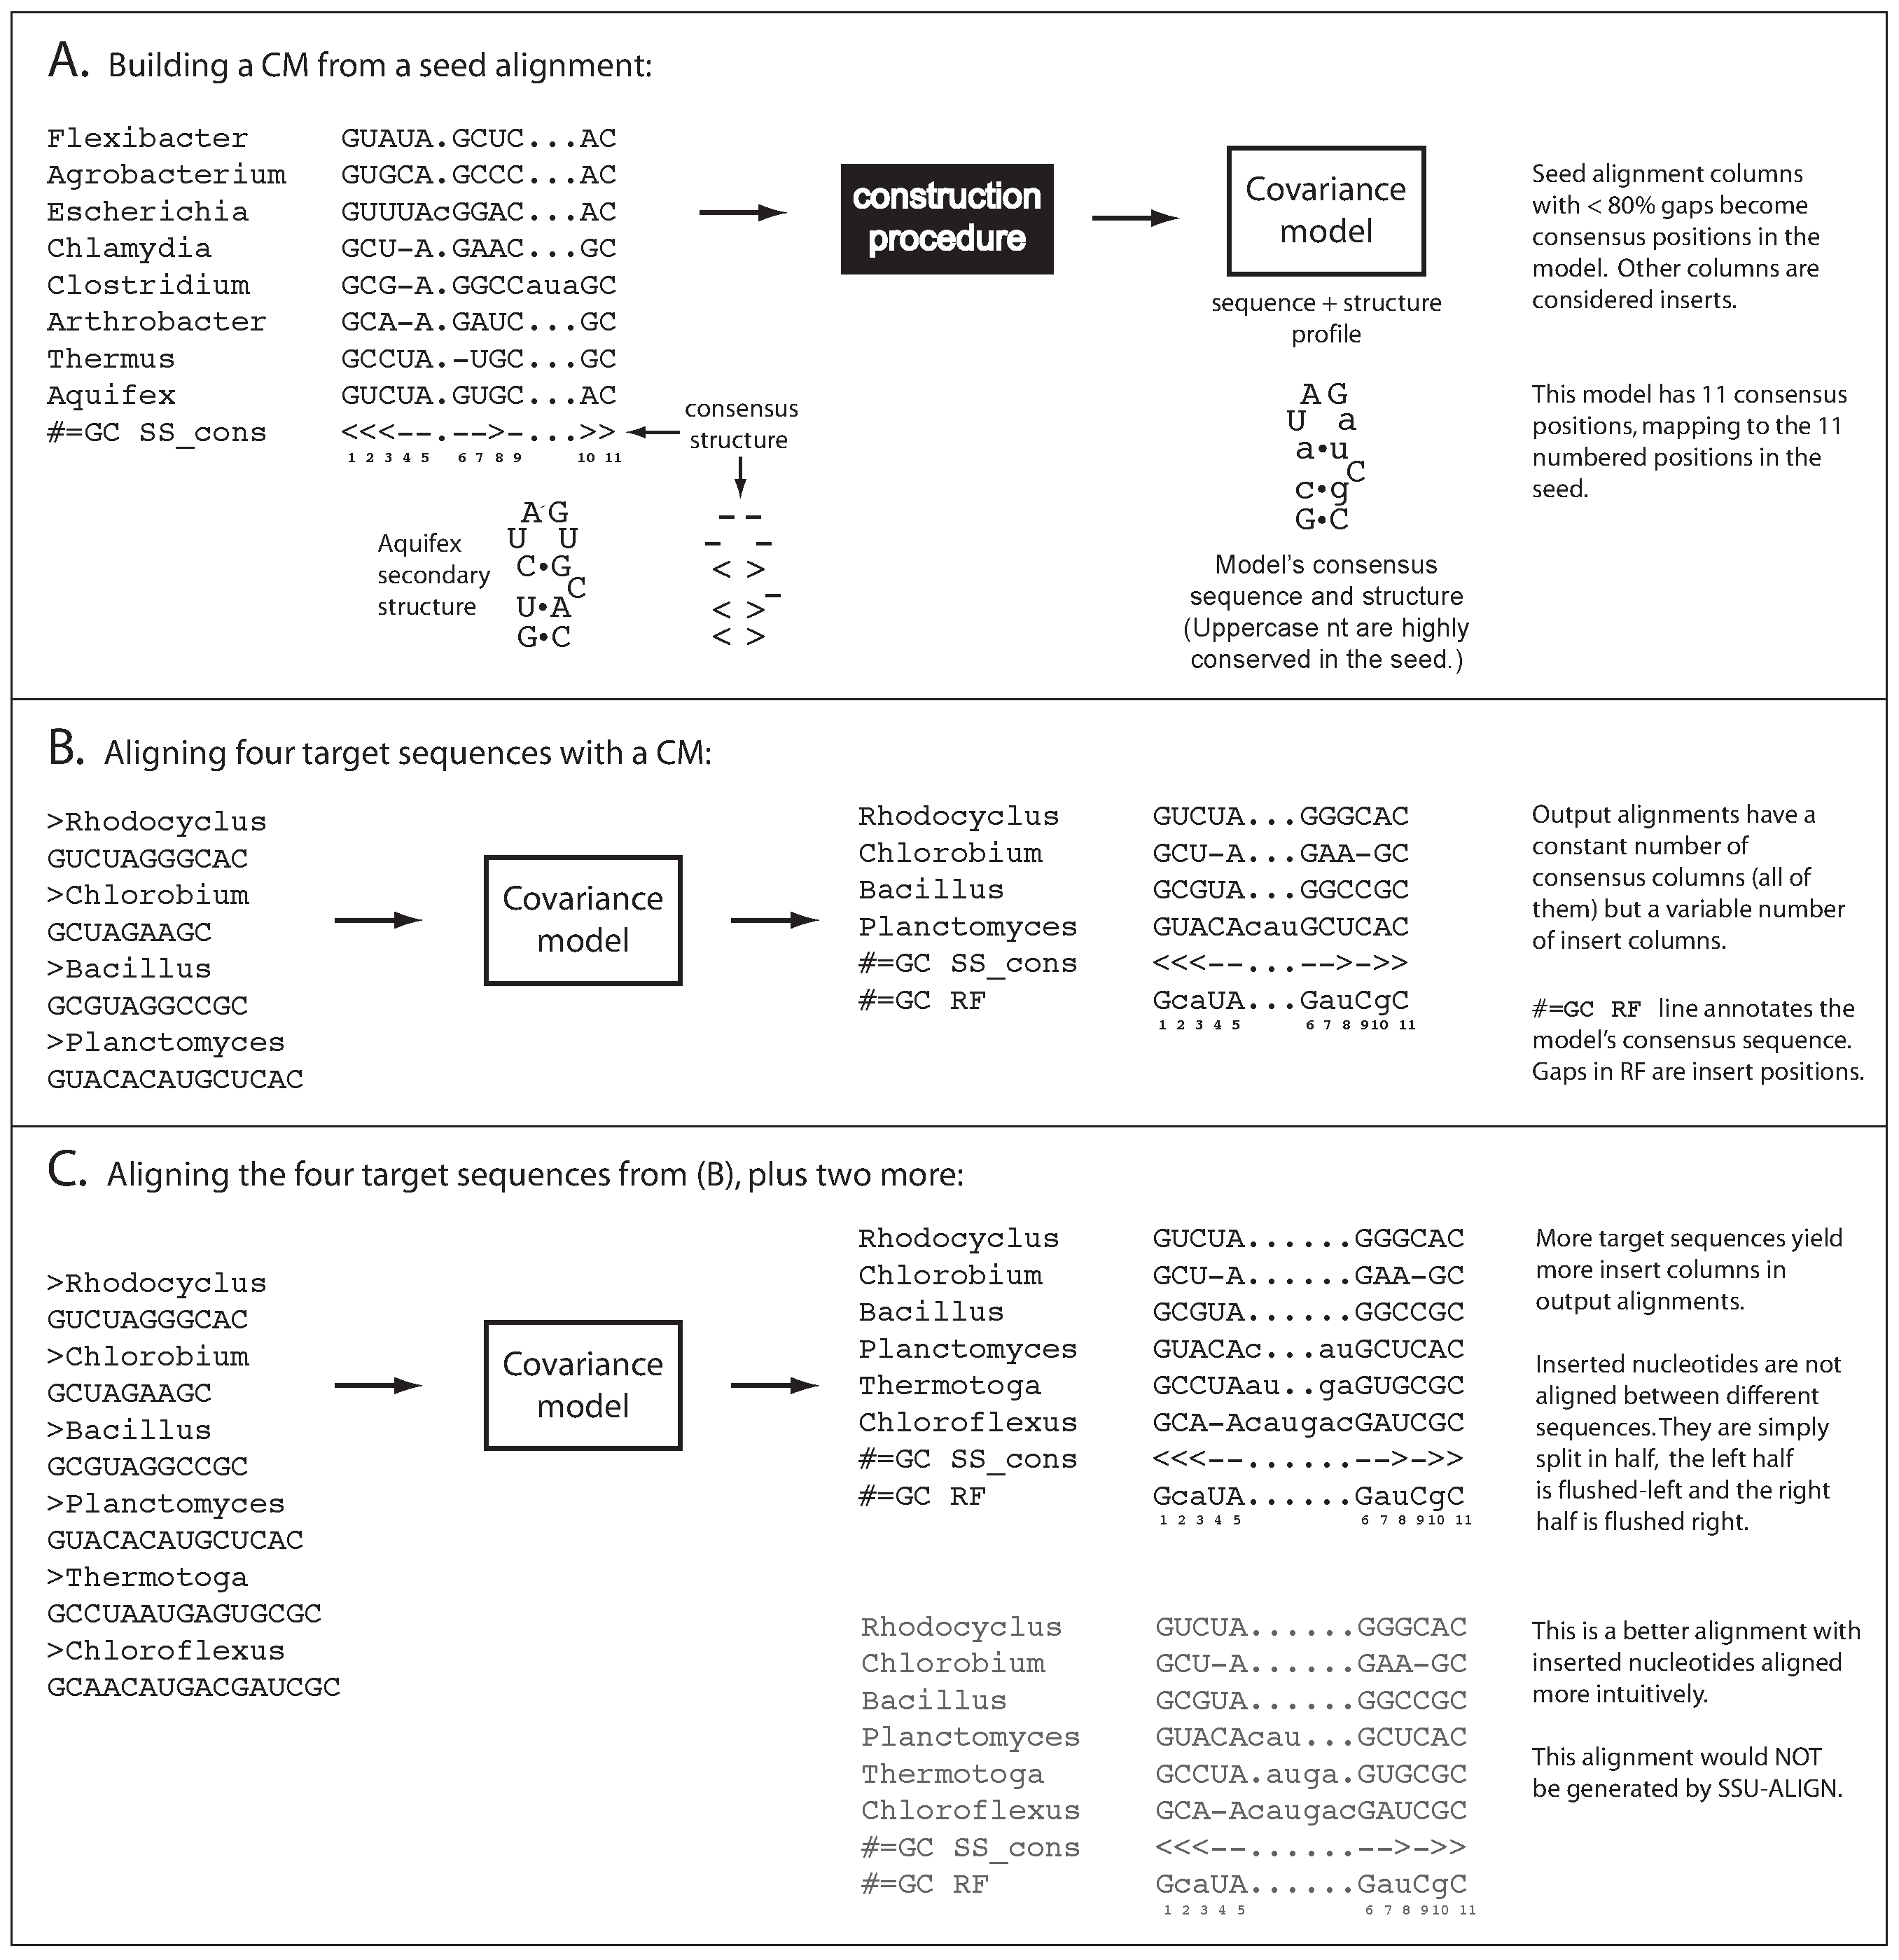
\includegraphics[height=7in]{Figures/sa-toy-example}
\caption{Building and aligning sequences to an example CM.}
\end{center}
\label{fig:toyex}
\end{figure}


\subsection{Automated probabilistic alignment masking}

The goal of masking is to identify and remove columns containing
nucleotides that are ambiguously aligned and therefore likely to contain
errors prior to using the alignment for phylogenetic inference.  Two
commonly used SSU masks were determined manually by David Lane and
Phil Hugenholtz (Figures 7.5 and 7.6 of \cite{Nawrocki09b}) based on
expert knowledge and extensive experience with SSU alignments.
Alignment posterior probabilities from
probabilistic models offer an alternative, objective way of evaluating
alignment ambiguity (high posterior probability means low ambiguity
and vice versa) and creating masks for any alignment.

%This is in the thesis, but it is irrelevant here.
\begin{comment}
The HMM banded alignment technique described in Chapter 8 of
\cite{Nawrocki09b} exploits
posterior probabilities calculated from the Forward and Backward
algorithms in HMM alignments. Inside and Outside, the
SCFG analogs of the Forward and Backward, can be used to calculate
posterior probabilities for CM alignment \cite{Durbin98}. These
algorithms were not implemented in \sft{infernal} prior to this work
because they are about two-fold slower than the (already slow) CYK
algorithm and because the Myers-Miller linear memory trick that made
CM SSU alignment practical (requiring 60 Mb instead of 20 Gb of RAM)
had only been applied to CYK \cite{Eddy02b}. HMM banding drastically
reduces the memory requirement for CM alignment, because only DP cells
within the bands need be allocated, making it possible to run Inside
and Outside on SSU.
\end{comment}

\subsubsection{Alignment ambiguity and length heterogeneity}

Alignment ambiguity often arises in regions of alignments with low
sequence conservation where insertions and deletions are common,
corresponding to regions of the molecule that exhibit high length
heterogeneity across different species. In such cases, it is often
difficult to determine the correct alignment because alternative
alignments seem plausible. Take for example the CM alignment
of the {\tt GUAU} subsequence of the \emph{Desulfovibrio
desulfuricans} SSU sequence to a loop region depicted in
Figure~\ref{fig:ambiguity}. The reference (consensus) sequence for the
loop ({\tt AUUCAAC}) differs from {\tt GUAU} in both sequence and
length. Consequently, the CM alignment for this loop is not well
defined, and two alternative alignments are given posterior
probabilities above $0.35$.  In contrast, the surrounding helix
region, for which higher sequence similarity exists between the two
sequences, is aligned confidently with high posterior probabilities.

\begin{figure}
\ttfamily
\footnotesize
\begin{center}
%ORIGINAL DATA is from Macbook: 
%/Users/nawrockie/school/notebook/9_0309_ths/latex/ssu/ambiguity_example
\begin{tabular}{ll}
00904::Desulfovibrio\_desulfuricans-1 &                         GAUGUCGGGGA--GUAU---UCUUCGGUGUC \\
\#=GR 00904::Desulfovibrio\_desulfuricans-1 PP &                ***********--6666---9********** \\
& \\
00904::Desulfovibrio\_desulfuricans-2          &                GAUGUCGGGGA---GUAU--UCUUCGGUGUC \\
\#=GR 00904::Desulfovibrio\_desulfuricans-2 PP &                ***********---4444--9********** \\
& \\
\#=GC SS\_cons                        &                             <<<<<<<<<<<<.......>>>>>>>>>>>> \\
\#=GC RF                              &                             GGUGUuGGgggcAuUcaACgcccUCaGUGCC \\
\end{tabular}
\rmfamily

\vspace{0.2in}
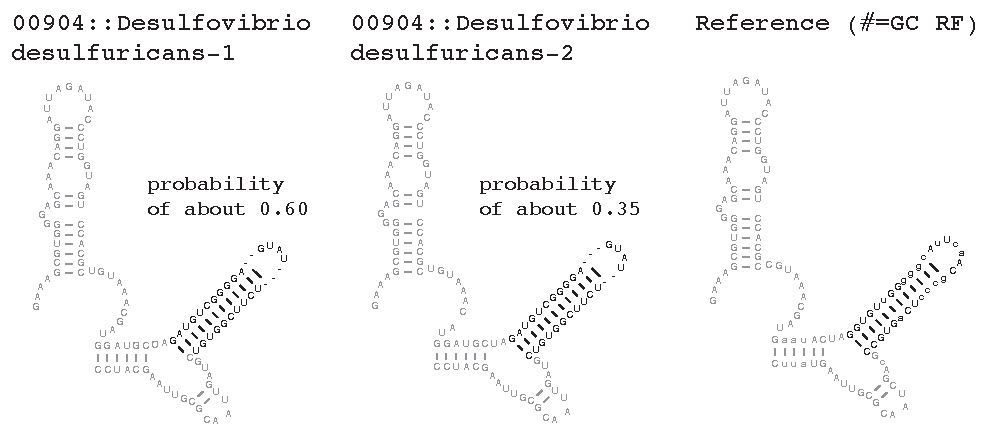
\includegraphics[width=5.7in]{Figures/ambiguity}

\caption[Example of alignment ambiguity in a hairpin loop.]{
  \textbf{Example of alignment ambiguity in a hairpin loop.}  Top: An
  alignment fragment of two different alignments of the
  \emph{Desulfovibrio desulfuricans} (sequence accession
  \texttt{M34113}) sequence from the \sft{ssu-align} bacterial seed
  alignment for the region between consensus columns $861$ and $881$.
  Each alignment is annotated with its posterior probability in the
  \texttt{\#=GR PP} rows.  Characters in PP rows have 12 possible
  values: "0-9", "*", or ".". If ".", the position corresponds to a
  gap in the sequence. A value of "0" indicates a posterior
  probability of between 0.0 and 0.05, "1" indicates between 0.05 and
  0.15, "2" indicates between 0.15 and 0.25 and so on up to "9" which
  indicates between 0.85 and 0.95. A value of "*" indicates a
  posterior probability of between 0.95 and 1.0. Higher posterior
  probabilities correspond to greater confidence that the aligned
  nucleotide belongs where it appears in the alignment.  For example,
  the second \texttt{A} in the first aligned sequence has a PP value
  of '6' indicating a posterior probability of between 0.55 and 0.65
  of being aligned in its current position. The
  probability this \texttt{A} aligns in the next position over, as it
  does in the second alignment, is between 0.35 and 0.45 as indicated
  by the 4 in that position.  The \texttt{\#=GC
  SS\_cons} and \texttt{\#=GC RF} rows correspond to the consensus
  secondary structure and sequence respectively.  
%The alignments were
%  created using \texttt{cmalign} to align this sequence to the
%  bacterial CM with the \texttt{--sample} option.  
  Bottom: The
  secondary structures corresponding to the two possible alignments of
  the \emph{D. desulfuricans} and the reference alignment.  Nucleotides
  in the actual alignment are black. Nucleotides surrounding the
  alignment fragment are gray.}
\end{center}
\label{fig:ambiguity}
\end{figure}


\subsection{Other useful references}

The \software{infernal} user's guide \cite{infernalguide} included in
this package supplements this user's guide. My Ph.D. thesis 
(\htmladdnormallink{http://selab.janelia.org/publications.html}{http://selab.janelia.org/publications.html})
introduces and describes my work on CM methods. It includes three chapters (7-9) dedicated to
SSU rRNA alignment; chapter 9 is included in this guide as
section~\ref{section:chap9}, but the other chapters may include some
relevant background information as well. 
Other useful references on CMs include
\cite{Eddy94,Eddy02b,NawrockiEddy07,Nawrocki09,KolbeEddy09}. In
addition, the \database{rfam} database 
(\htmladdnormallink{http://rfam.sanger.ac.uk/}{http://rfam.sanger.ac.uk/})
uses \software{infernal} to search for and align
structural RNAs using more than 1000 different CMs, so its
publications may be of interest as well
\cite{Griffiths-Jones03,Griffiths-Jones05,Gardner09}.

